\section{Results}
\label{results}

All three methods are evaluated over 315 route trials on Town05. Table~\ref{tab:main-results} summarizes the aggregate metrics, while Figs.~\ref{fig:collision-breakdown}--\ref{fig:infraction-breakdown} visualize the score distributions and per-class collision breakdown.

\begin{table*}[!htbp]
\centering
\caption{Aggregate evaluation results on Town05 (315 trials each; driving score shown with 95\% CI). Collision columns are split by actor class: vehicles, bicycles, and pedestrians.}
\label{tab:main-results}
{\scriptsize
\setlength{\tabcolsep}{5.5pt}
\begin{tabular}{lcccccccccc}
\toprule
\textbf{Method}
  & \makecell{\textbf{Driving}\\\textbf{Score\,$\uparrow$}}
  & \makecell{\textbf{Route}\\\textbf{Score\,$\uparrow$}}
  & \makecell{\textbf{Route}\\\textbf{Compl.\,$\uparrow$}}
  & \makecell{\textbf{Coll.}\\\textbf{/Route\,$\downarrow$}}
  & \makecell{\textbf{Coll.}\\\textbf{/km\,$\downarrow$}}
  & \makecell{\textbf{Coll.}\\\textbf{Free\,$\uparrow$}}
  & \makecell{\textbf{Veh.}\\\textbf{/Rt\,$\downarrow$}}
  & \makecell{\textbf{Bike}\\\textbf{/Rt\,$\downarrow$}}
  & \makecell{\textbf{Ped.}\\\textbf{/Rt\,$\downarrow$}}
  & \makecell{\textbf{Static}\\\textbf{/Rt\,$\downarrow$}} \\
\midrule
PID-only
  & 45.47\,($\pm$4.41)
  & 96.91
  & 90.2\%
  & 2.952
  & 35.58
  & 31.7\%
  & 0.968
  & 1.527
  & 0.390
  & 0.067 \\
Fixed CBF
  & 67.39\,($\pm$3.58)
  & 95.36
  & 88.3\%
  & 0.784
  & 9.56
  & 48.6\%
  & 0.168
  & 0.286
  & 0.302
  & 0.029 \\
\textbf{Adaptive CBF}
  & \textbf{75.81}\,($\pm$3.35)
  & 96.71
  & \textbf{90.8\%}
  & \textbf{0.581}
  & \textbf{6.75}
  & \textbf{59.7\%}
  & 0.187
  & \textbf{0.187}
  & \textbf{0.178}
  & 0.029 \\
\bottomrule
\end{tabular} }
\end{table*}

%------------------------------------------------------------------
\subsection{Safety Analysis}
%------------------------------------------------------------------

As shown in Table~\ref{tab:main-results}, the adaptive CBF policy scores 75.81\,($\pm$\,3.35) on the driving metric and produces the fewest collisions across bicycles and pedestrians. Relative to PID-only, total collisions per route drop by 80.3\% (2.952 to 0.581), and collisions per kilometer by 81.0\% (35.58 to 6.75), with bicycles seeing the steepest reduction at 87.7\% (1.527 to 0.187). Vehicle and pedestrian collisions fall by 80.7\% (0.968 to 0.187) and 54.5\% (0.390 to 0.178), respectively.


The adaptive policy further improves on the fixed CBF baseline, cutting collisions per route by 25.9\% (0.784 to 0.581) and collisions per kilometer by 29.3\% (9.56 to 6.75). Most of this improvement comes from pedestrians (41.1\% lower) and bicycles (34.4\% lower), which aligns with the design intent: the RL policy raises $\gamma_p$ and $\gamma_b$ when vulnerable road users approach the ego trajectory, braking more aggressively only when it matters. The collision-free route rate rises from 48.6\% under fixed CBF to 59.7\% under the adaptive CBF. Fig.~\ref{fig:collision-breakdown} shows the per-class breakdown. PID-only's total is dominated by bicycle collisions, which account for over half of its bar. Both CBF methods reduce bicycle and vehicle collisions substantially, bringing those categories to comparable levels. The adaptive policy then separates itself from the fixed variant primarily through lower pedestrian collisions, consistent with its ability to tighten $\gamma$ when vulnerable road users are nearby.


%------------------------------------------------------------------
\subsection{Efficiency Analysis}
%------------------------------------------------------------------

Despite being more conservative on safety, the adaptive policy does not sacrifice route progress. It slightly edges out PID-only route completion (90.8\% vs.\ 90.2\%), while fixed CBF completes only 88.3\%. The fixed gain tends to over-brake in tight gaps, stalling the vehicle; the adaptive policy avoids this by relaxing $\gamma$ when no hazard is nearby, so it records only 24 blocked-agent failures versus 35 for fixed CBF and 31 for PID-only. The penalty factor (driving score divided by route score) captures how cleanly routes are completed: 0.784 for adaptive policy, 0.707 for fixed CBF, and 0.469 for PID-only. In other words, PID-only loses more than half its route score to infraction penalties on an average run.


%------------------------------------------------------------------
\subsection{Score Distribution}

%------------------------------------------------------------------

The violin plots in Fig.~\ref{fig:overall-scores} give a fuller picture than the averages alone. The black line represents the mean, and the red line represents the median. More than half of the adaptive CBF routes (56.2\%) score a perfect 100, pulling the median to 100.0. Fixed CBF sits at a median of 60.0 and PID-only at 30.0; the latter shows a heavy lower tail with 85 routes below a score of 10, each flagging an early collision that dominates the final penalty. The tighter interquartile range for adaptive policy ($[50, 100]$ versus $[8, 100]$ for PID-only) suggests that improvement holds in a wide variety of route layouts rather than being concentrated on a few easy ones. Route-level paired comparisons support this: the adaptive policy outscores PID-only on 64.4\% of routes (worse on only 7.9\%) and beats fixed CBF on 36.2\% (worse on 18.7\%).

%------------------------------------------------------------------
\subsection{Infraction Breakdown}
%------------------------------------------------------------------

Fig.~\ref{fig:infraction-breakdown} breaks down the mean infractions per route in the five categories shown. Bicycle infractions are the largest for PID-only at 1.527 per route; fixed CBF reduces this to 0.286, and the adaptive policy to 0.187. Vehicle infractions follow a similar trend: 0.968 for PID-only, 0.168 for fixed CBF, and 0.187 for adaptive. Pedestrian infractions drop from 0.390 (PID-only) to 0.302 (fixed CBF) and 0.178 (adaptive). Static object infractions are low across the board -- 0.067, 0.029, and 0.029 for PID-only, fixed CBF, and adaptive, respectively. Stop-sign infractions round out the picture at 0.248 for PID-only, 0.235 for fixed CBF, and 0.168 for the adaptive policy.


\begin{figure}[!htbp]
  \centering
  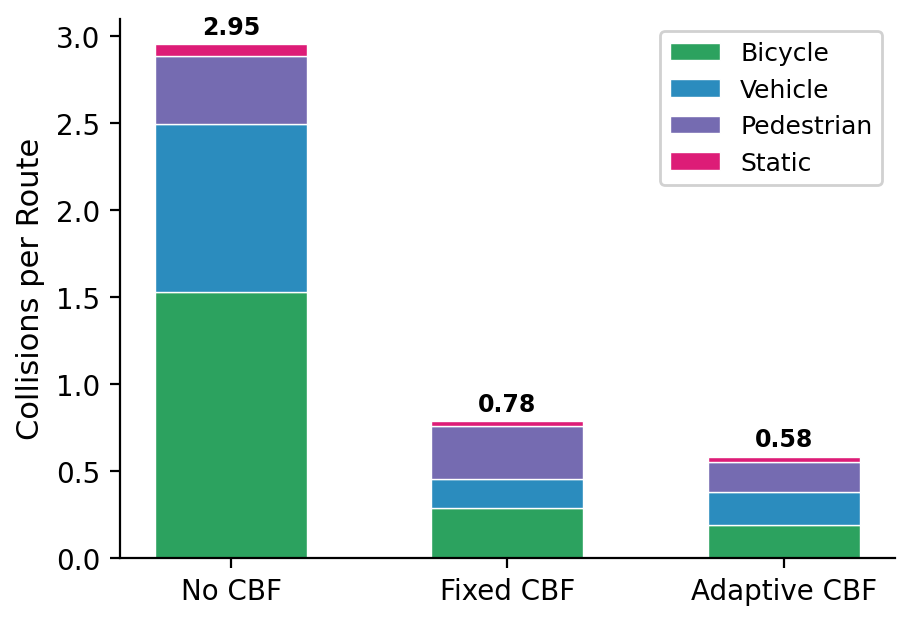
\includegraphics[width=0.5\columnwidth]{figures/collision_breakdown.png}
  \caption{Mean collisions per route, stacked by actor class.}
  \label{fig:collision-breakdown}
\end{figure}

\begin{figure}[!htbp]
  \centering
  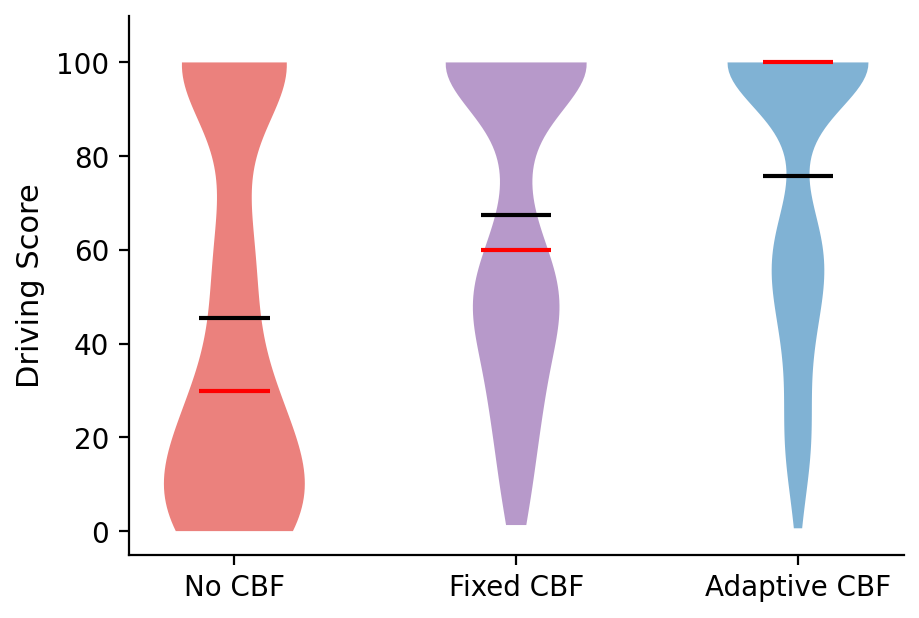
\includegraphics[width=0.5\columnwidth]{figures/score_distribution.png}
  \caption{Per-route driving score distributions.}
  \label{fig:overall-scores}
\end{figure}



\begin{figure}[!htbp]
  \centering
  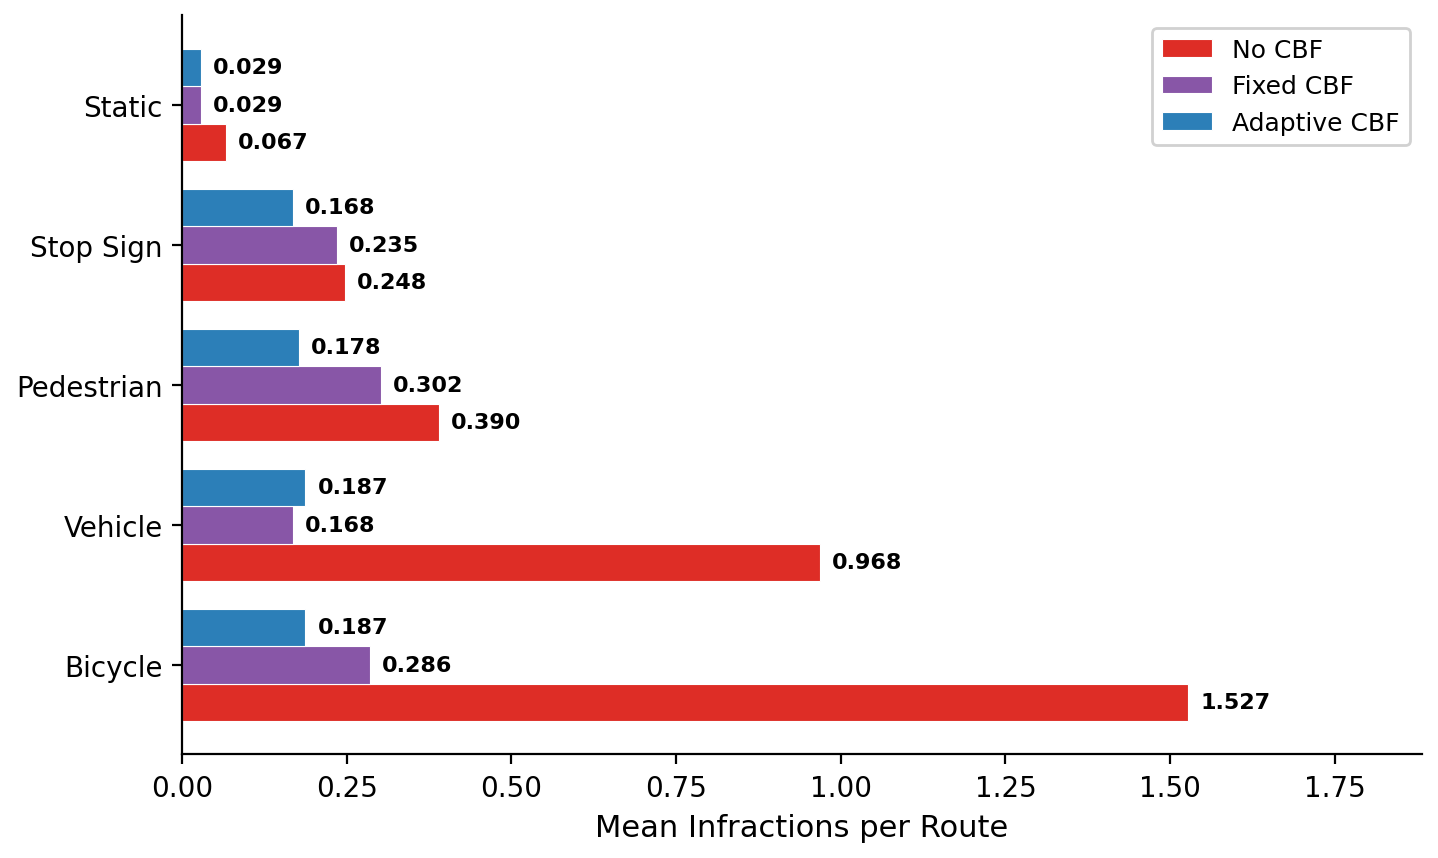
\includegraphics[width=0.9\columnwidth]{figures/all_infractions_per_route.png}
  \caption{Mean infractions per route by category.}
  \label{fig:infraction-breakdown}
\end{figure}

%------------------------------------------------------------------
\subsection{Execution Time and Constraint Activation}
\label{sec:solve-time}
%------------------------------------------------------------------

Across the full evaluation matrix ($\sim$42k decision steps per method), the OSQP solve for a single decision step averages $0.017$\,ms (95th percentile $0.041$\,ms, maximum $<\!1.1$\,ms), against the $200$\,ms budget imposed by the $5$\,Hz decision rate -- solve time consumes under $0.02\%$ of the available budget on average, well within real-time requirements even in dense traffic. The QP's slack variable is active on $30.4\%$ of decision steps for the fixed-gain baseline and $35.2\%$ for the adaptive policy, indicating the soft constraint is exercised regularly rather than only in rare edge cases; the solver never fell back to the nominal (unfiltered) command in either case ($0.0\%$ fallback rate across both methods), so feasibility was never lost even under the one-step linearization discussed in Section~\ref{methods}.

%------------------------------------------------------------------
\subsection{Fixed-Gain Sensitivity Sweep}
\label{sec:gamma-sweep}
%------------------------------------------------------------------

Table~\ref{tab:gamma-sweep} sweeps the fixed-CBF gain across its full configured range. The eight fixed-gain points span only $66.55$--$71.75$, a band narrower than any individual point's own 95\% CI ($\pm6.2$--$6.6$) -- no fixed gain is statistically distinguishable from any other, indicating the fixed-CBF baseline was not tuned to an unfavorable operating point. At matched sample size ($\gamma{=}0.5$ vs.\ adaptive, both $n{=}315$), the adaptive policy's advantage is real but modest: $75.81\pm3.35$ vs.\ $67.39\pm3.58$, confidence intervals barely non-overlapping. Fig.~\ref{fig:gamma-pareto} plots this as a Pareto frontier.

\begin{table}[!htbp]
\centering
\caption{Fixed-CBF gamma sensitivity sweep, Town05 ($n{=}105$ per point except $\gamma{=}0.5$, $n{=}315$).}
\label{tab:gamma-sweep}
{\scriptsize
\setlength{\tabcolsep}{4pt}
\begin{tabular}{lcccc}
\toprule
$\gamma$ & Score & 95\% CI & Compl. & Coll./km \\
\midrule
0.1 & 67.76 & 6.51 & 90.5\% & 10.76 \\
0.2 & 69.64 & 6.23 & 88.6\% & 8.98 \\
0.3 & 67.55 & 6.22 & 88.6\% & 8.95 \\
0.4 & 71.75 & 6.31 & 86.7\% & 8.49 \\
0.5 & 67.39 & 3.58 & 88.3\% & 9.56 \\
0.6 & 66.57 & 6.65 & 86.7\% & 11.46 \\
0.7 & 70.54 & 6.42 & 89.5\% & 9.42 \\
0.8 & 66.55 & 6.62 & 89.5\% & 10.43 \\
\textbf{Adaptive} & \textbf{75.81} & 3.35 & 90.8\% & 6.75 \\
\bottomrule
\end{tabular} }
\end{table}

\begin{figure}[!htbp]
  \centering
  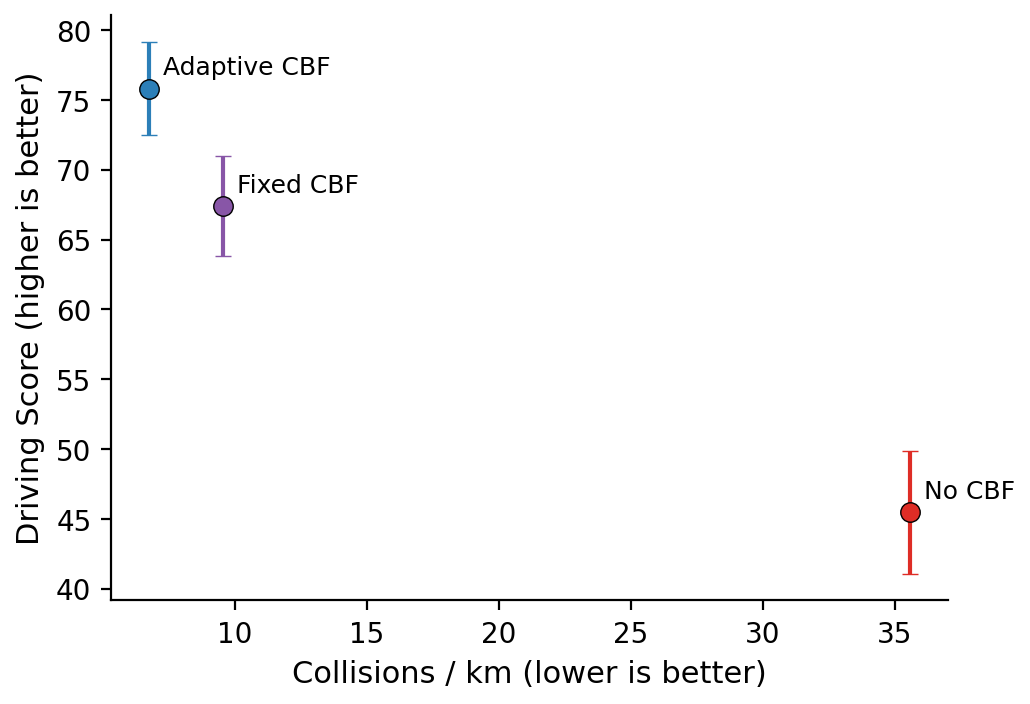
\includegraphics[width=0.9\columnwidth]{figures/pareto_score_vs_collisions.png}
  \caption{Fixed-CBF gamma sweep: score vs.\ collision rate, adaptive CBF shown as reference.}
  \label{fig:gamma-pareto}
\end{figure}

%------------------------------------------------------------------
\subsection{Cross-Map Generalization}
\label{sec:generalization}
%------------------------------------------------------------------

Table~\ref{tab:generalization} evaluates the frozen trained policy zero-shot on two held-out towns. The CBF-vs-no-CBF safety benefit holds cleanly across all three towns: PID-only's collision rate rises sharply out of distribution ($35.58\rightarrow99.57\rightarrow66.13$ per km) while both CBF variants remain in a comparatively narrow band. The adaptive-over-fixed advantage observed on Town05, however, does not generalize: the two are statistically indistinguishable on Town07, and fixed CBF outperforms the adaptive policy on Town10 on both score and collision rate. We report this directly: the safety-layer concept generalizes, but the specific claim that adaptive scheduling outperforms a well-tuned fixed gain is currently supported only in-distribution.

\begin{table}[!htbp]
\centering
\caption{Cross-map generalization, zero-shot (no retraining).}
\label{tab:generalization}
{\scriptsize
\setlength{\tabcolsep}{4pt}
\begin{tabular}{lccc}
\toprule
Method & Town05 ($n{=}315$) & Town07 ($n{=}42$) & Town10 ($n{=}27$) \\
\midrule
PID-only score      & 45.47$\pm$4.4  & 23.46$\pm$9.8 & 17.33$\pm$11.4 \\
Fixed CBF score      & 67.39$\pm$3.6  & 71.50$\pm$8.2 & 43.27$\pm$12.6 \\
Adaptive CBF score   & 75.81$\pm$3.4  & 72.86$\pm$8.9 & 38.41$\pm$12.6 \\
\midrule
PID-only coll./km    & 35.58 & 99.57 & 66.13 \\
Fixed CBF coll./km   & 9.56  & 9.50  & 14.37 \\
Adaptive CBF coll./km& 6.75  & 9.26  & 20.97 \\
\bottomrule
\end{tabular} }
\end{table}

%------------------------------------------------------------------
\subsection{Ablation Studies}
\label{sec:ablations}
%------------------------------------------------------------------

\textbf{Collaboration ablation.} Wrapping the identical safety layer around the single-agent (\texttt{no\_collaboration}) perception-planning checkpoint scores $67.57\pm6.52$, $89.5\%$ completion, $10.91$ collisions/km ($n{=}105$), versus $75.81\pm3.35$, $90.8\%$, $6.75$ with collaborative perception. The safety layer still delivers a large improvement over the unfiltered baseline without collaboration, but collaborative perception provides a further, meaningful benefit on top of it -- the reported gains are not solely an artifact of collaboration.

\textbf{Rule-based scheduler baseline.} Table~\ref{tab:rule-based} compares the hand-designed TTC-ramp scheduler against the other three methods. The ordering is monotonic on both score and collision rate: rule-based clearly beats no safety layer, but underperforms even the simplest fixed-gain CBF, and more so the learned adaptive policy -- the learned policy earns its added complexity over a simple hand-tuned rule.

\begin{table}[!htbp]
\centering
\caption{Rule-based (non-learned) gamma-scheduler baseline, Town05.}
\label{tab:rule-based}
{\scriptsize
\setlength{\tabcolsep}{4pt}
\begin{tabular}{lcccc}
\toprule
Method & $n$ & Score & Compl. & Coll./km \\
\midrule
PID-only        & 315 & 45.47$\pm$4.41 & 90.2\% & 35.58 \\
Rule-based CBF  & 105 & 64.46$\pm$6.76 & 89.5\% & 12.80 \\
Fixed CBF       & 315 & 67.39$\pm$3.58 & 88.3\% & 9.56 \\
Adaptive CBF    & 315 & 75.81$\pm$3.35 & 90.8\% & 6.75 \\
\bottomrule
\end{tabular} }
\end{table}

\textbf{Class-specific gain and observation-space proxies.} These are training-free proxies, not controlled ablations (Section~\ref{sec:additional-ablations}); we report them as such. Logging the trained policy's three gains over 6{,}485 decision steps shows they do not converge to a shared value: mean pairwise gaps of $0.60$--$0.63$ between the pedestrian gain and the other two classes, with $0\%$ of steps landing all three gains within even $0.10$ of each other -- the deployed policy clearly exploits class-specific freedom, particularly for pedestrians, though this does not establish that a policy trained under a shared-gain constraint could not perform comparably. One class's mean gain ($\gamma_v{=}0.800$, the top of the configured range) has exactly zero measured variance across all logged steps, which we note as a possible sign that this action dimension saturated during training rather than learning to differentiate, and flag as worth further investigation rather than presenting as a clean result. Separately, masking the heading-alignment features at inference dropped mean score from $67.73$ to $63.10$ and raised collisions from 14 to 18 over the same 20 routes, a real but noisy effect (6 routes worse, 4 better, 10 unchanged) consistent with the policy relying on this feature to some degree, though it cannot separate that from sensitivity to an out-of-distribution input.

%------------------------------------------------------------------
\subsection{Traffic Density and V2X Robustness}
\label{sec:robustness}
%------------------------------------------------------------------

On a 20-route subset (baseline: score $67.73$, $95\%$ completion, 14 collisions), $1.5\times$ denser traffic reduces the adaptive policy to score $61.09$, $70\%$ completion, 18 collisions -- a real degradation under harder conditions, as expected. Injected V2X communication latency ($400$\,ms) and collaborative-perception pose noise ($\sigma_{\text{pos}}{=}\sigma_{\text{rot}}{=}0.2$), tested individually, did not degrade score relative to baseline ($69.23$ and $73.42$ respectively). We report this as a single data point per condition rather than a sweep to a breaking point, and do not claim broad robustness from it alone.

\FloatBarrier